\section{Risultati Sperimentali}

    \begin{frame}{Esempi di Compressione}
        Esempi di compressione di un immagine a 24bpp del dataset Kodak\footnotemark[1] con le tecniche presentate\\
        \begin{figure}[!ht]
            \begin{minipage}[]{0.13\linewidth}
                \centering
                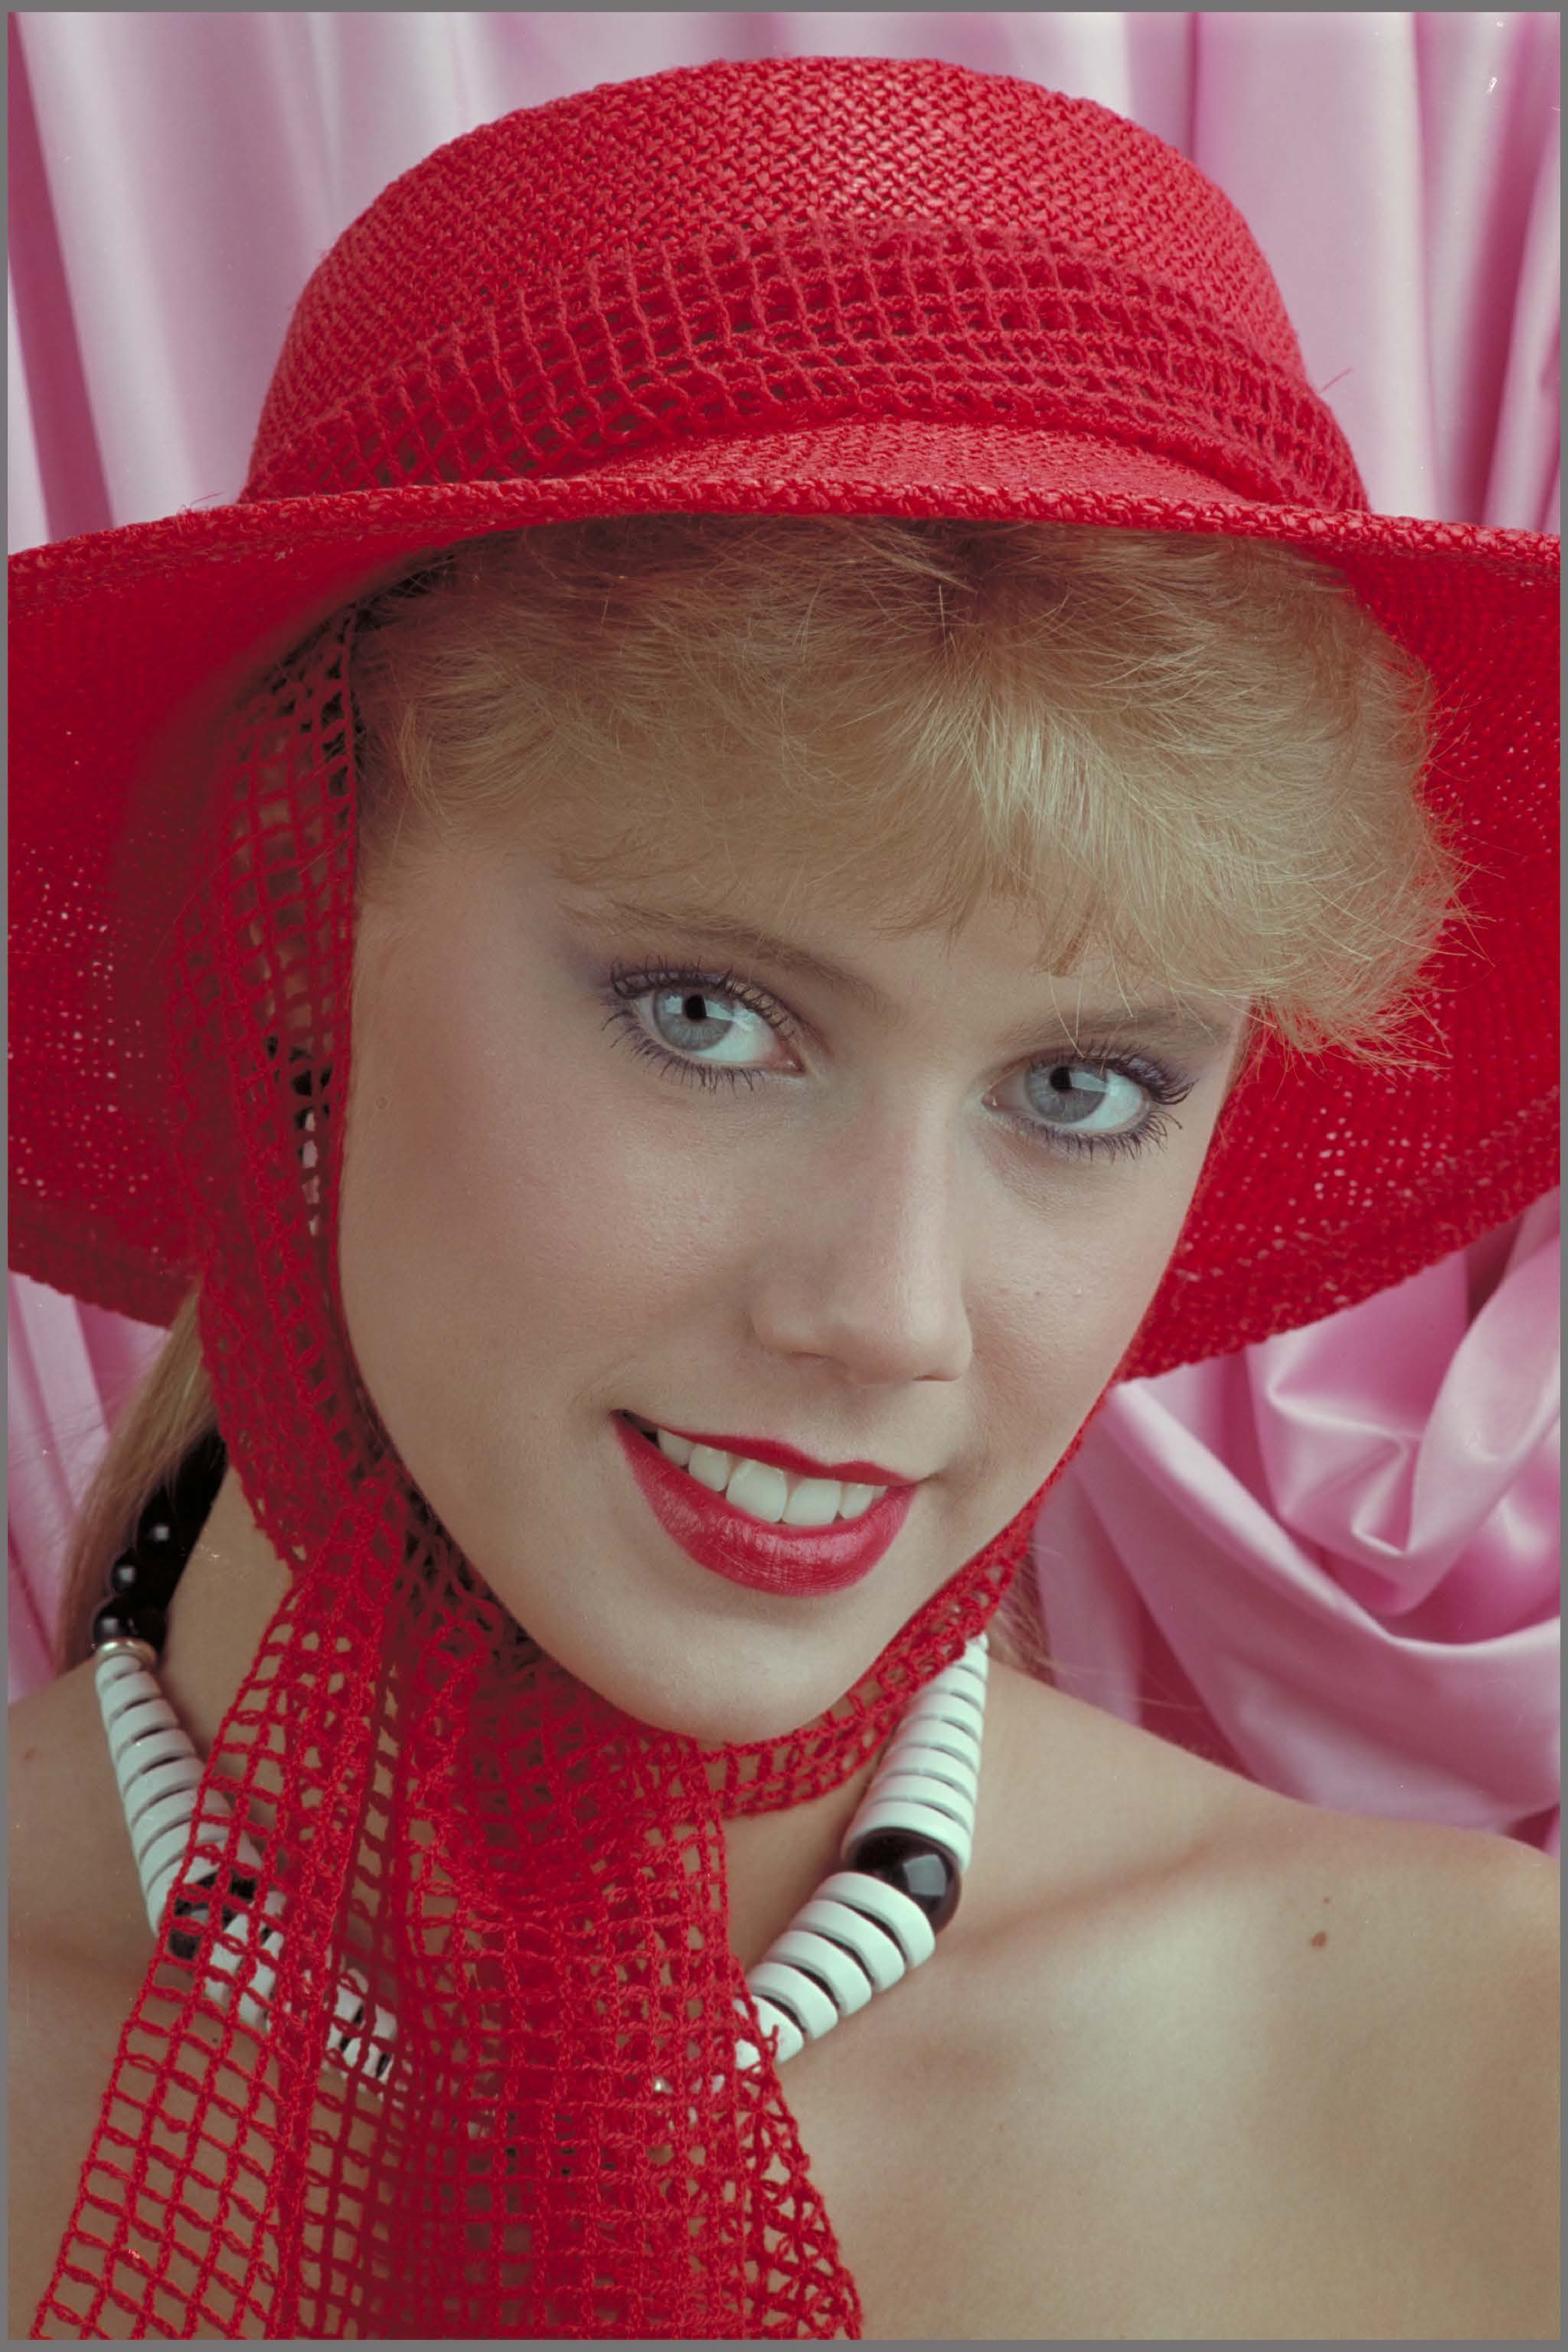
\includegraphics[width=\textwidth]{Immagini/IMAGES/PNG_IMG0004.pdf}
                \caption{Lossless 11.117bpp}
                \label{fig:Lossless}
            \end{minipage}
            \begin{minipage}[]{0.13\linewidth}
                \centering
                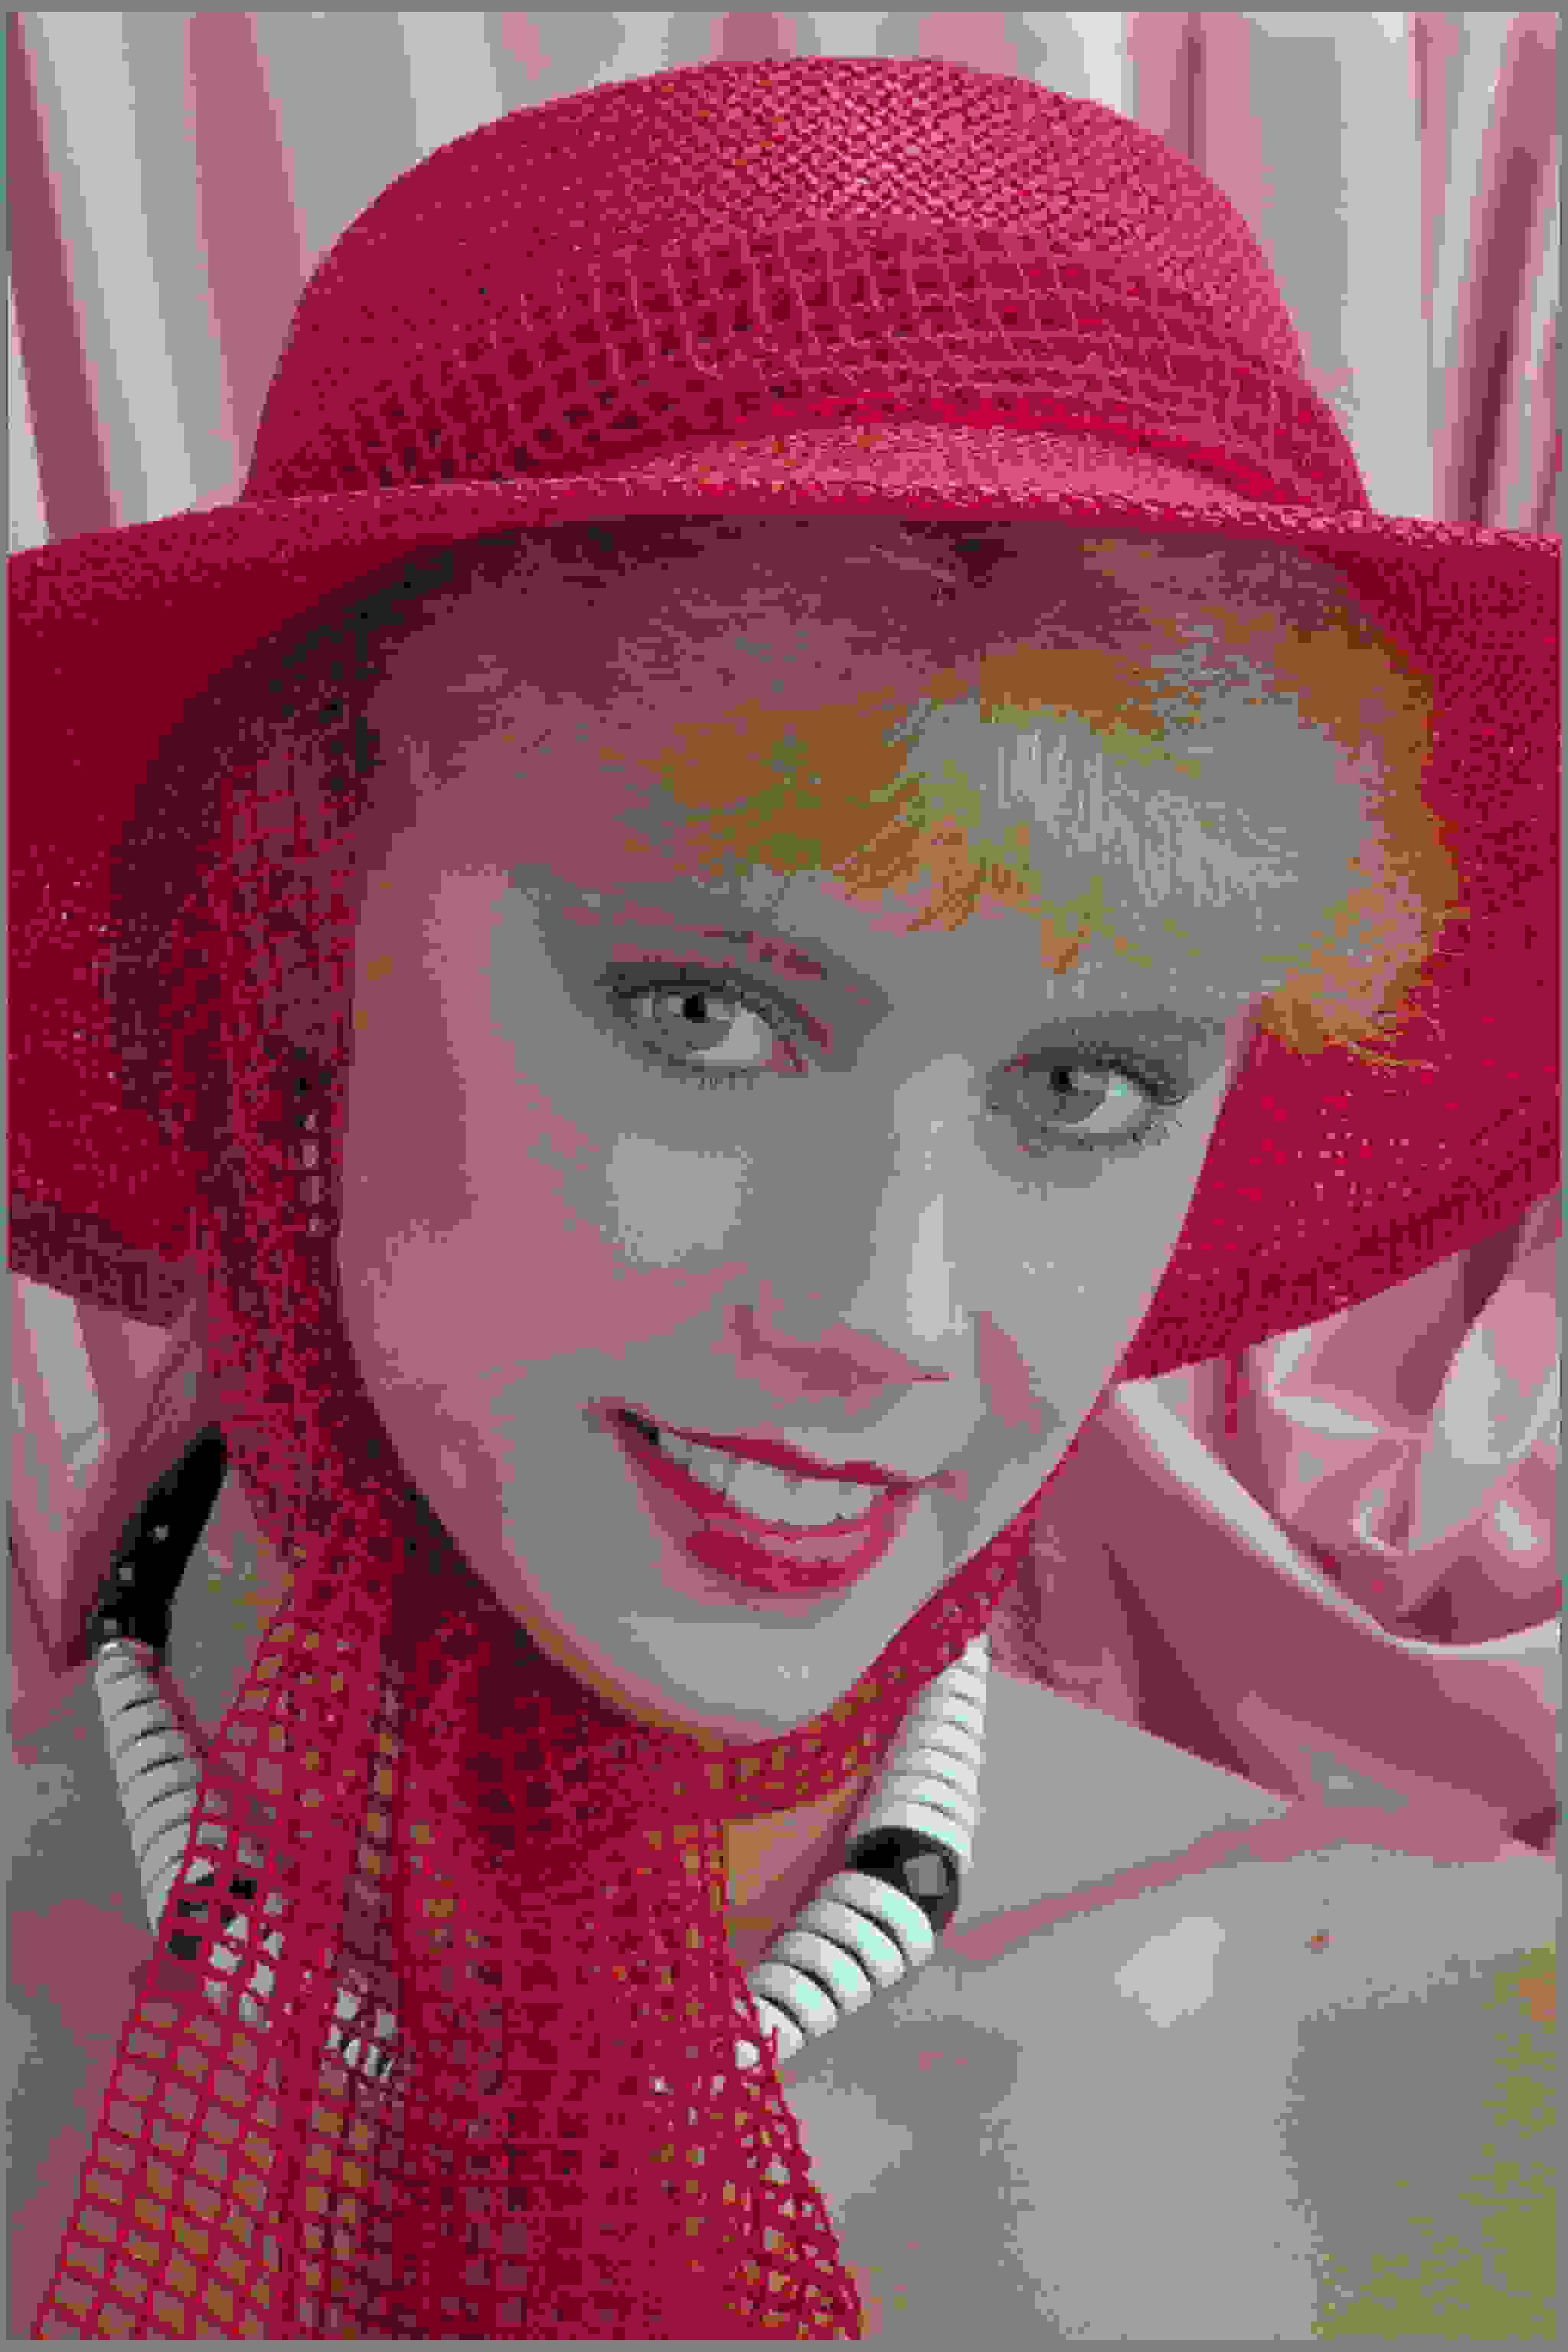
\includegraphics[width=\textwidth]{Immagini/IMAGES/JPEG_1_IMG0004.pdf}
                \caption{JPEG 0.167bpp}
                \label{fig:ExampleJPEG}
            \end{minipage}
            \begin{minipage}[]{0.13\linewidth}
                \centering
                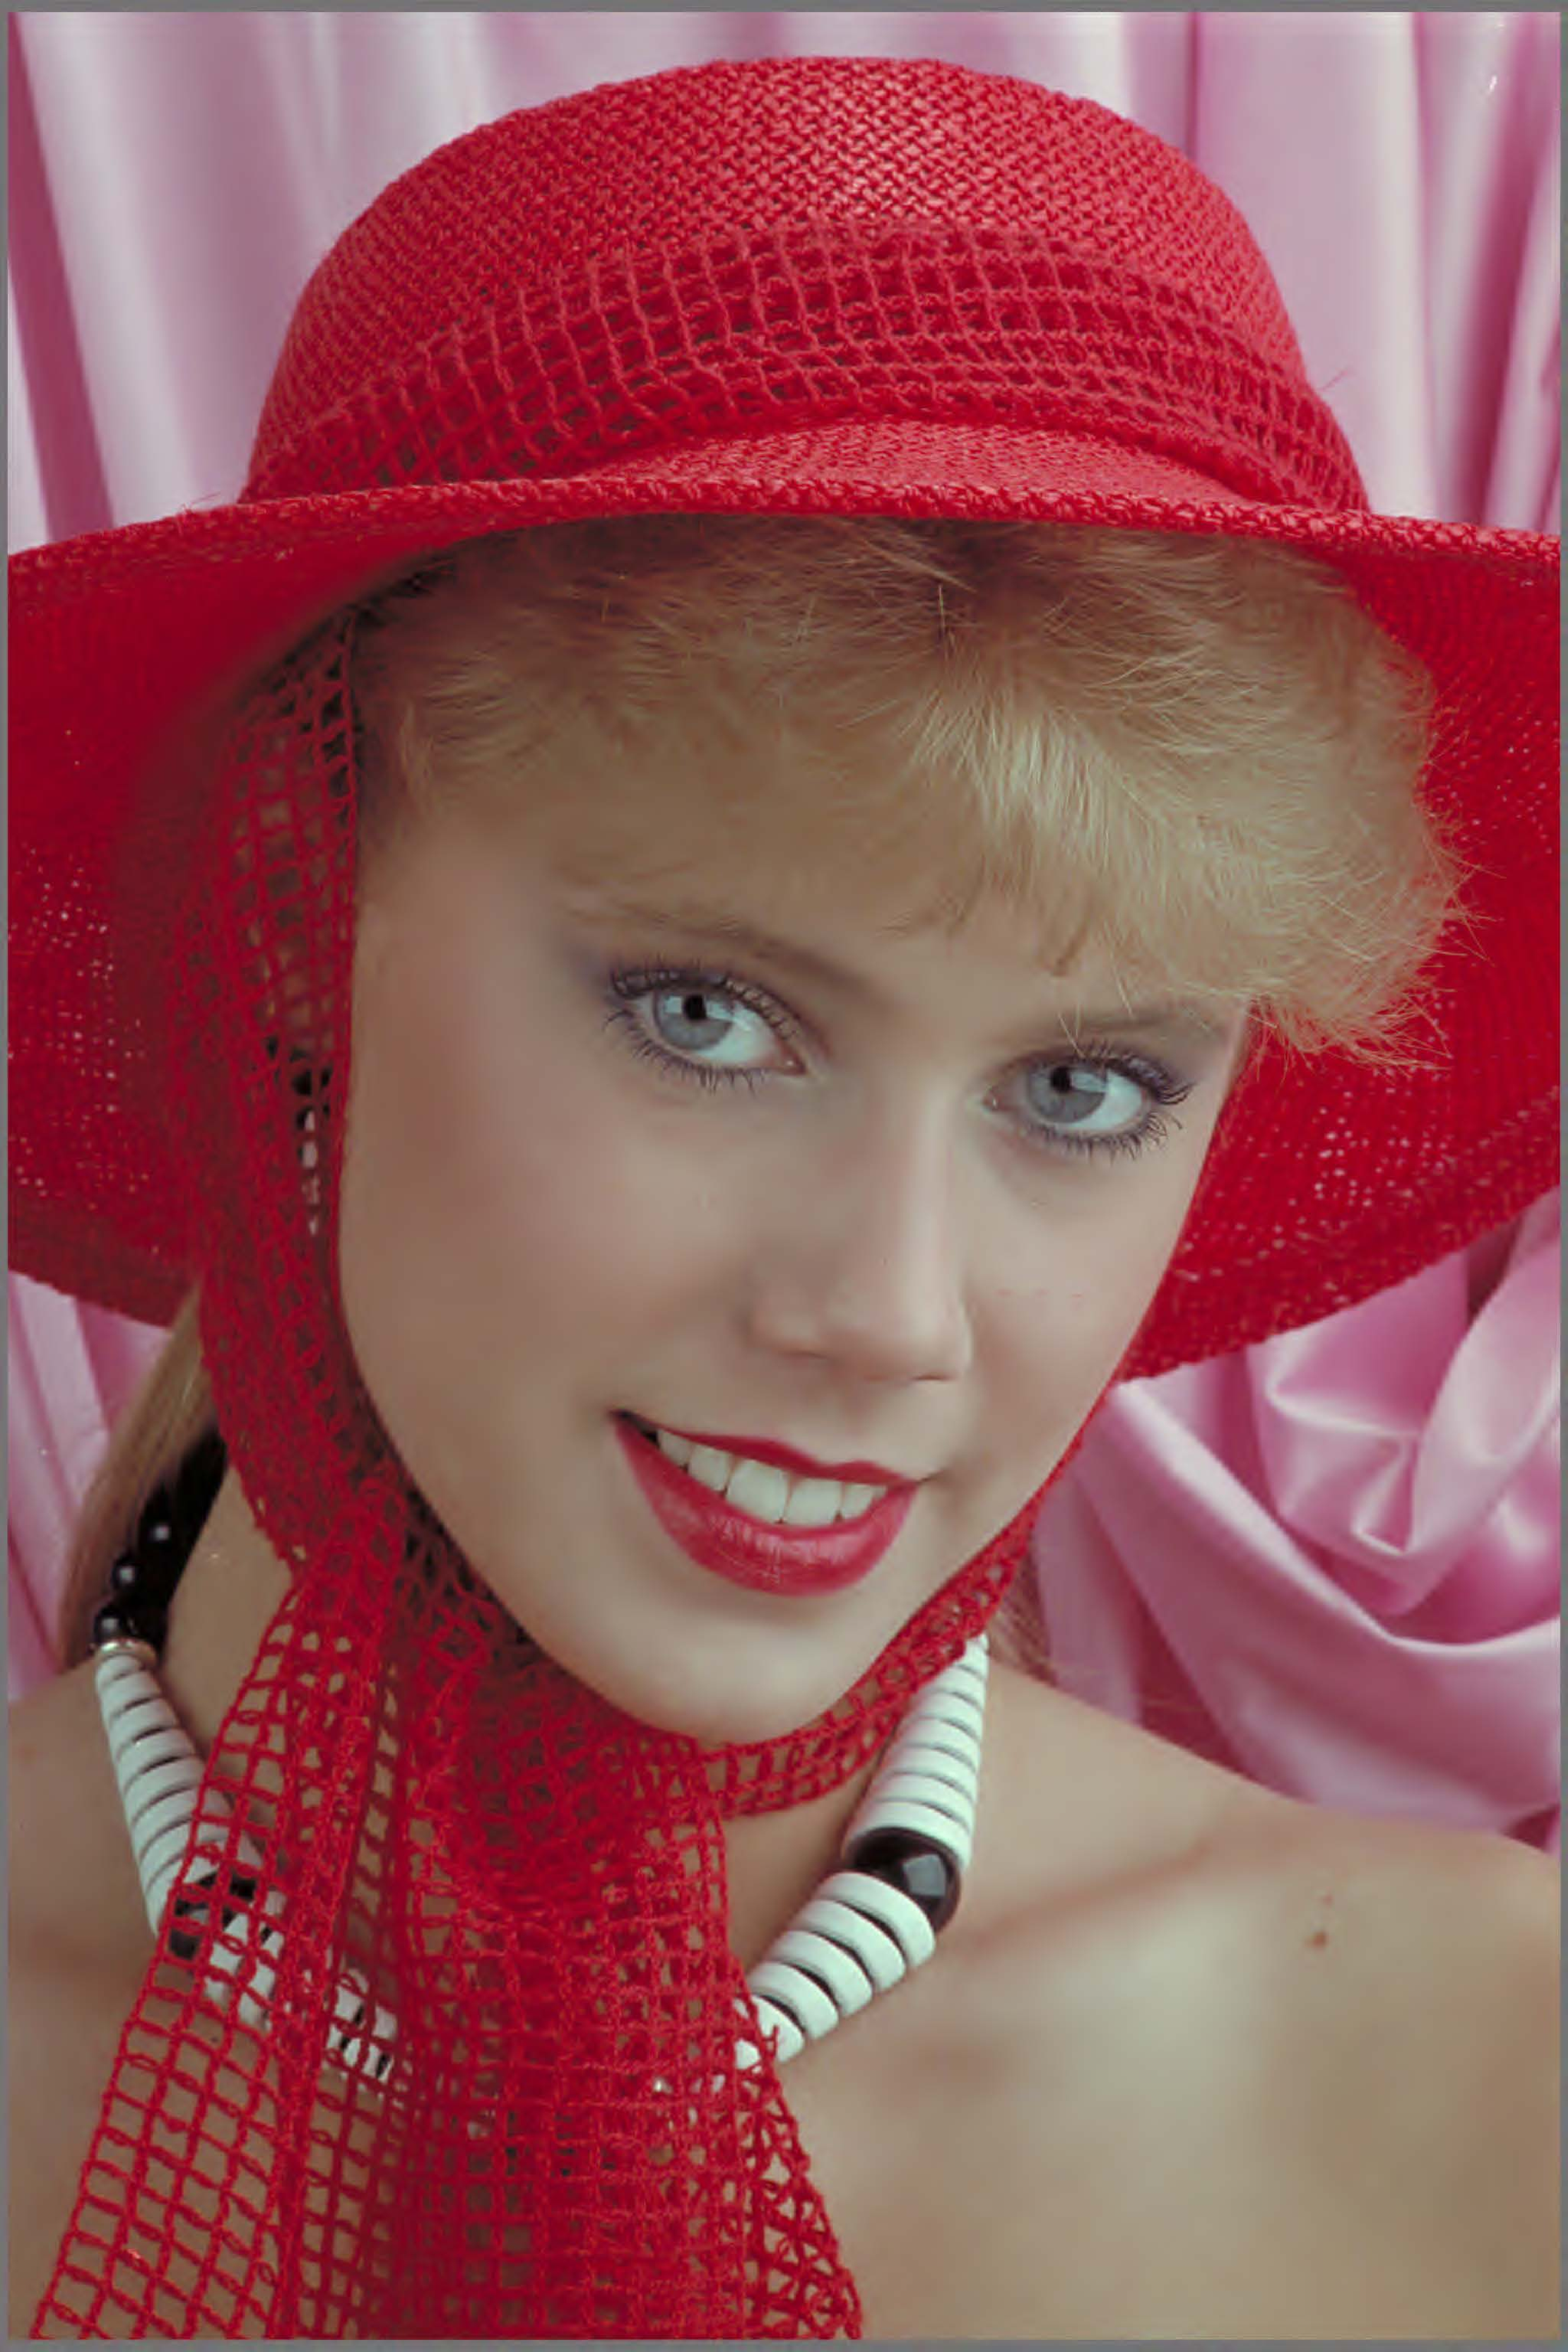
\includegraphics[width=\textwidth]{Immagini/IMAGES/JPEG2000_1_IMG0004.pdf}
                \caption{JPEG2000 0.137bpp}
                \label{fig:ExampleJPEG2000}
            \end{minipage}
            \begin{minipage}[]{0.13\linewidth}
                \centering
                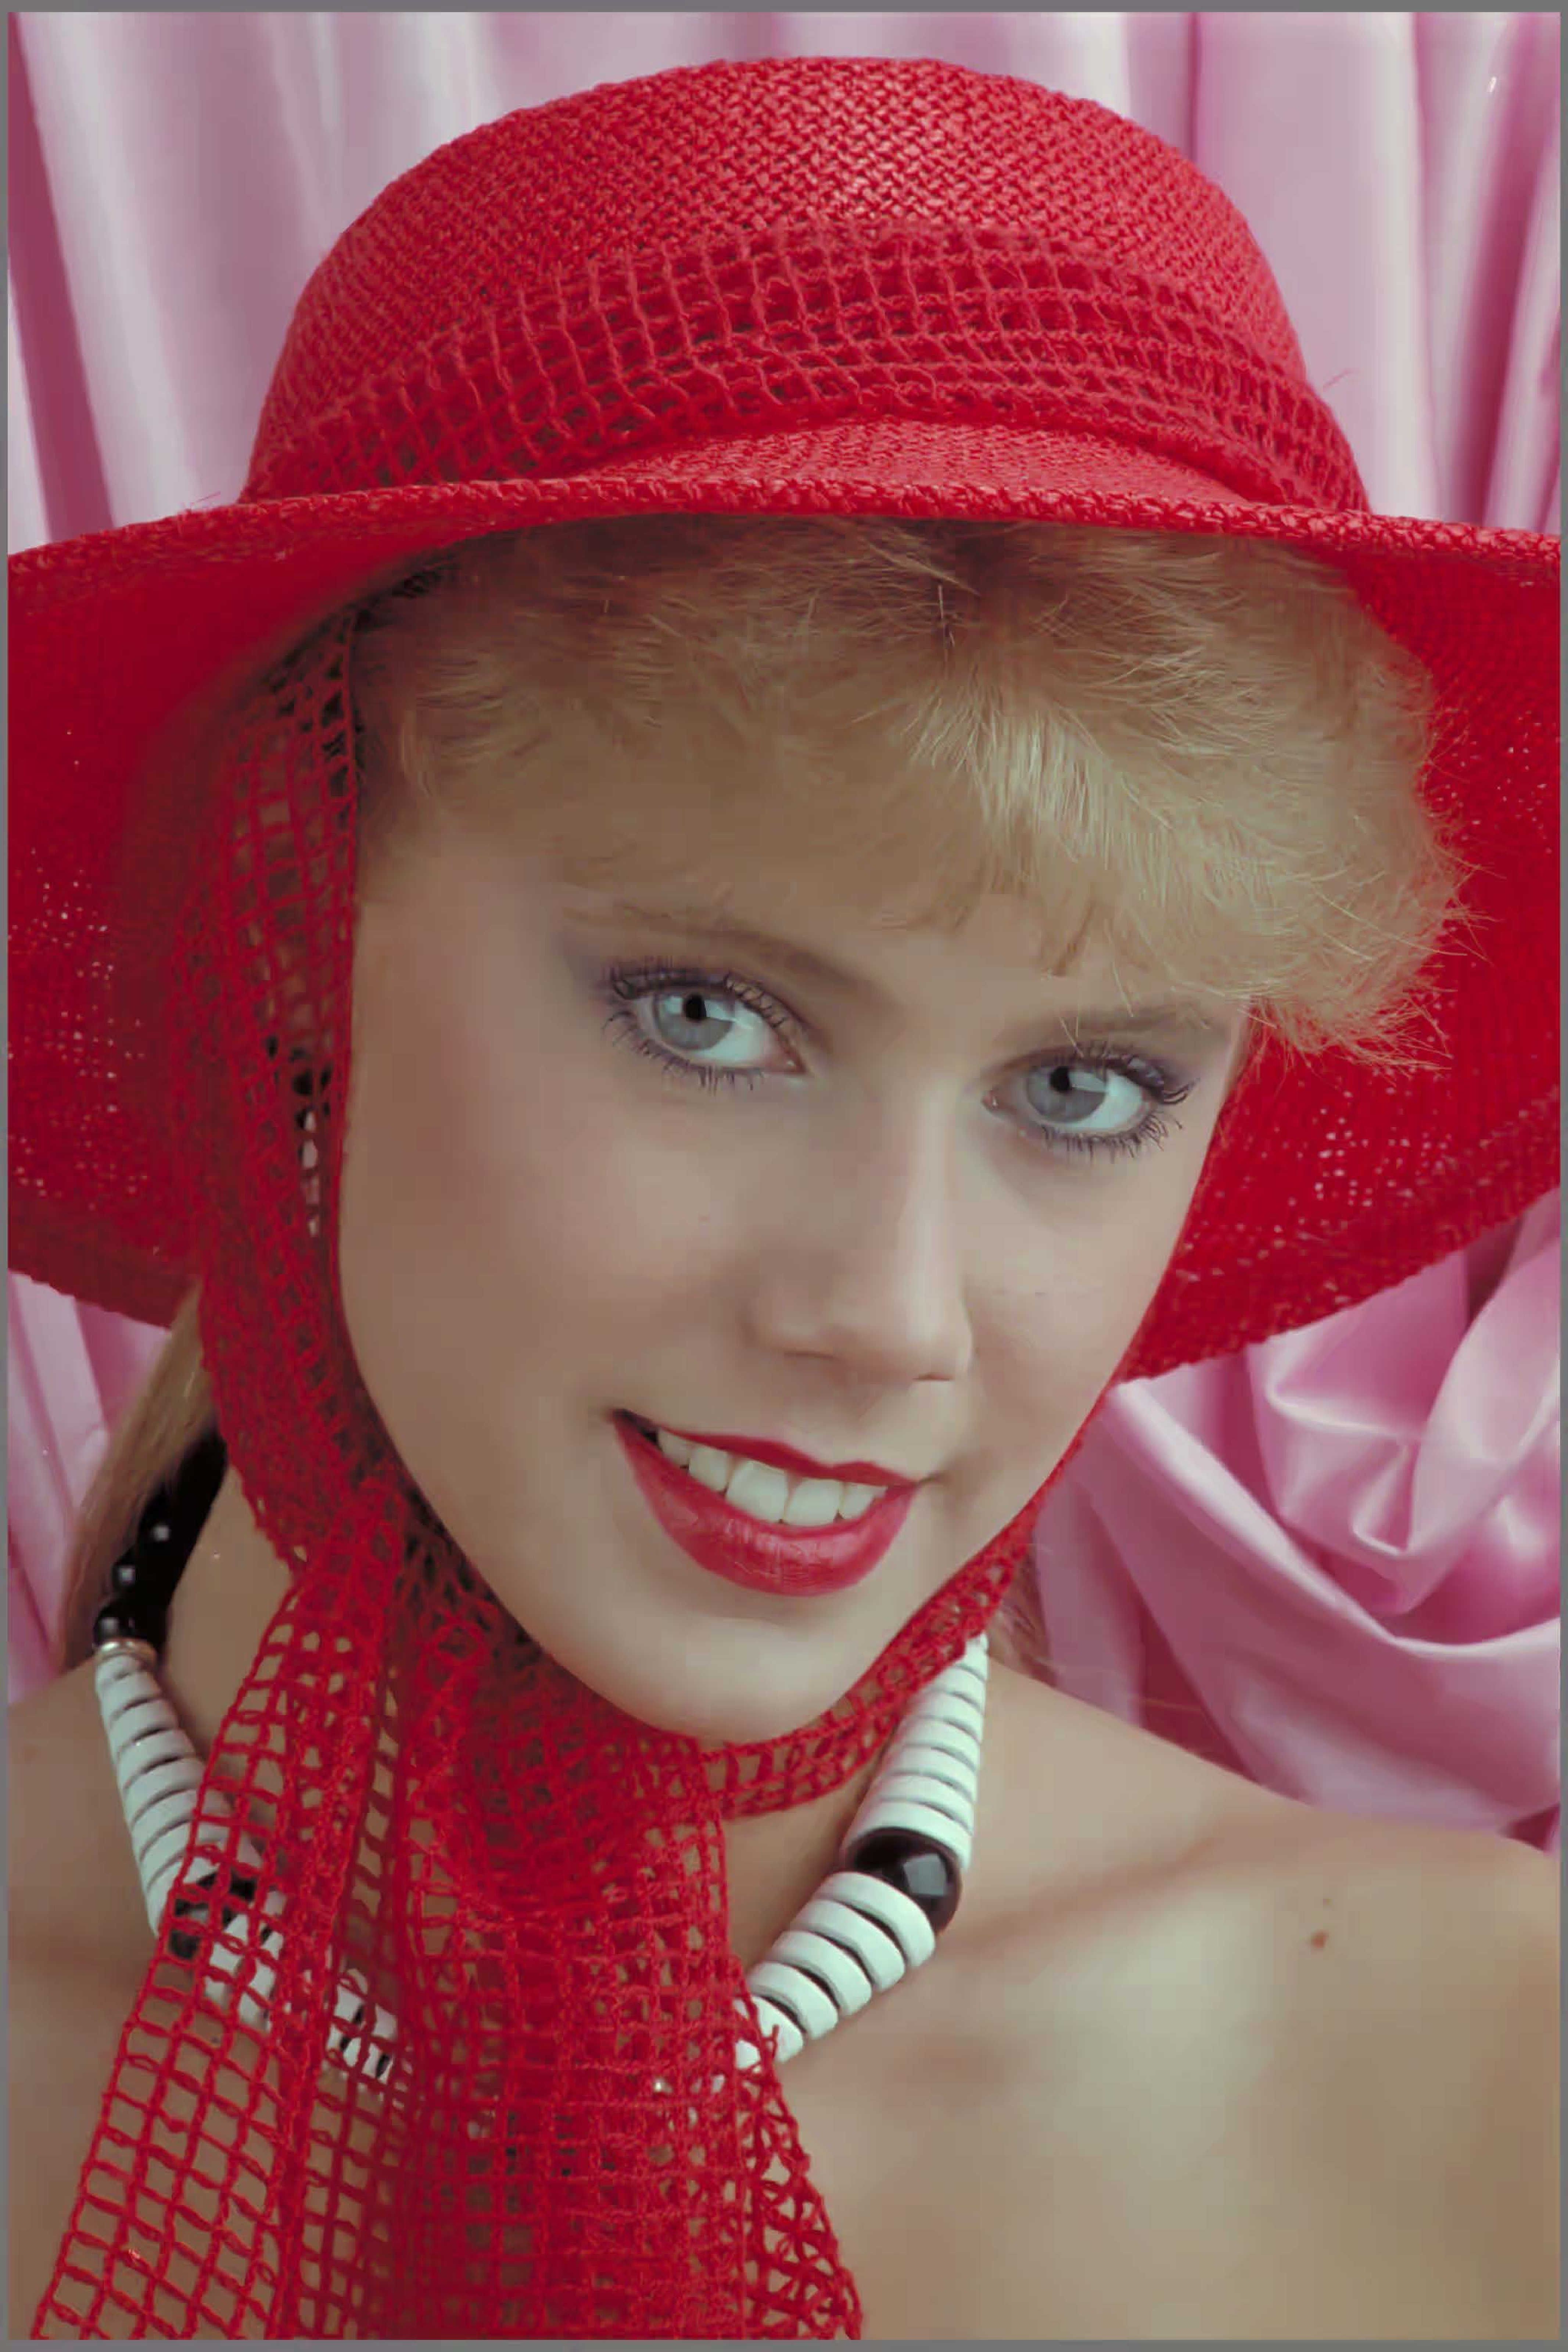
\includegraphics[width=\textwidth]{Immagini/IMAGES/BPG_2_IMG0004.pdf}
                \caption{BPG 0.103bpp}
                \label{fig:ExampleBPG}
            \end{minipage}
            \begin{minipage}[]{0.13\linewidth}
                \centering
                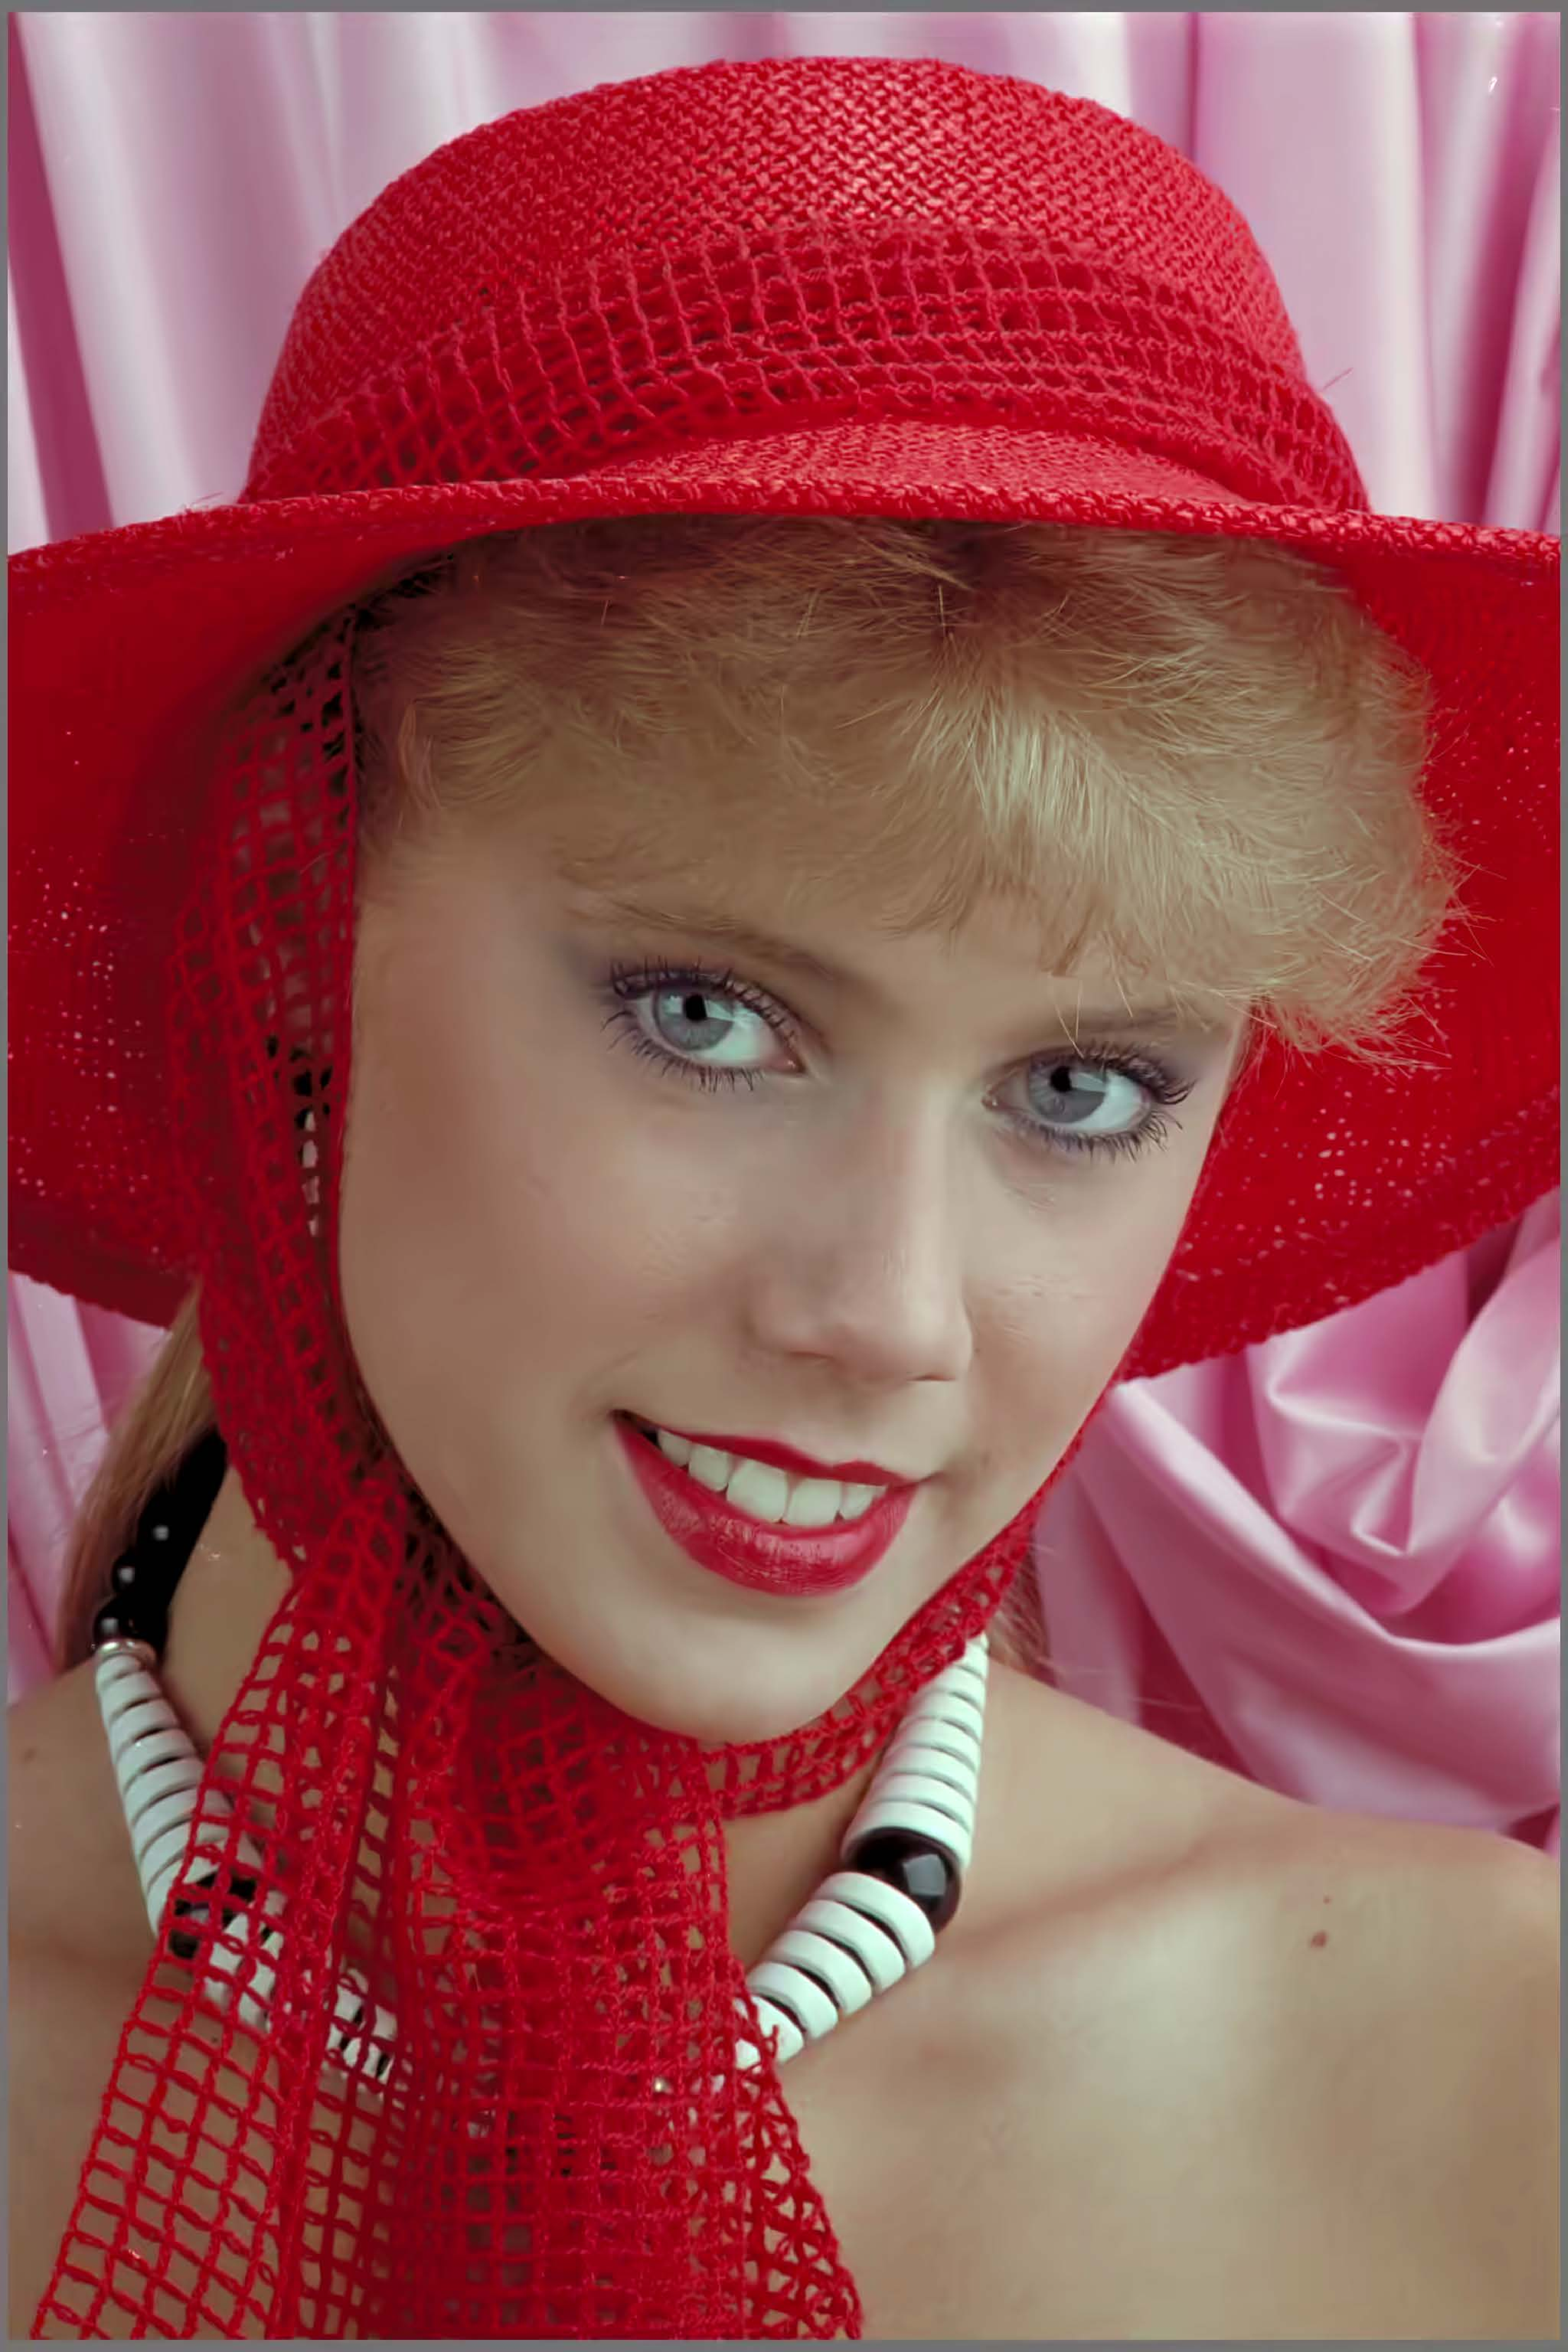
\includegraphics[width=\textwidth]{Immagini/IMAGES/VVC_1_IMG0004.pdf}
                \caption{VVC 0.061bpp}
                \label{fig:ExampleVVC}
            \end{minipage}
            \begin{minipage}[]{0.13\linewidth}
                \centering
                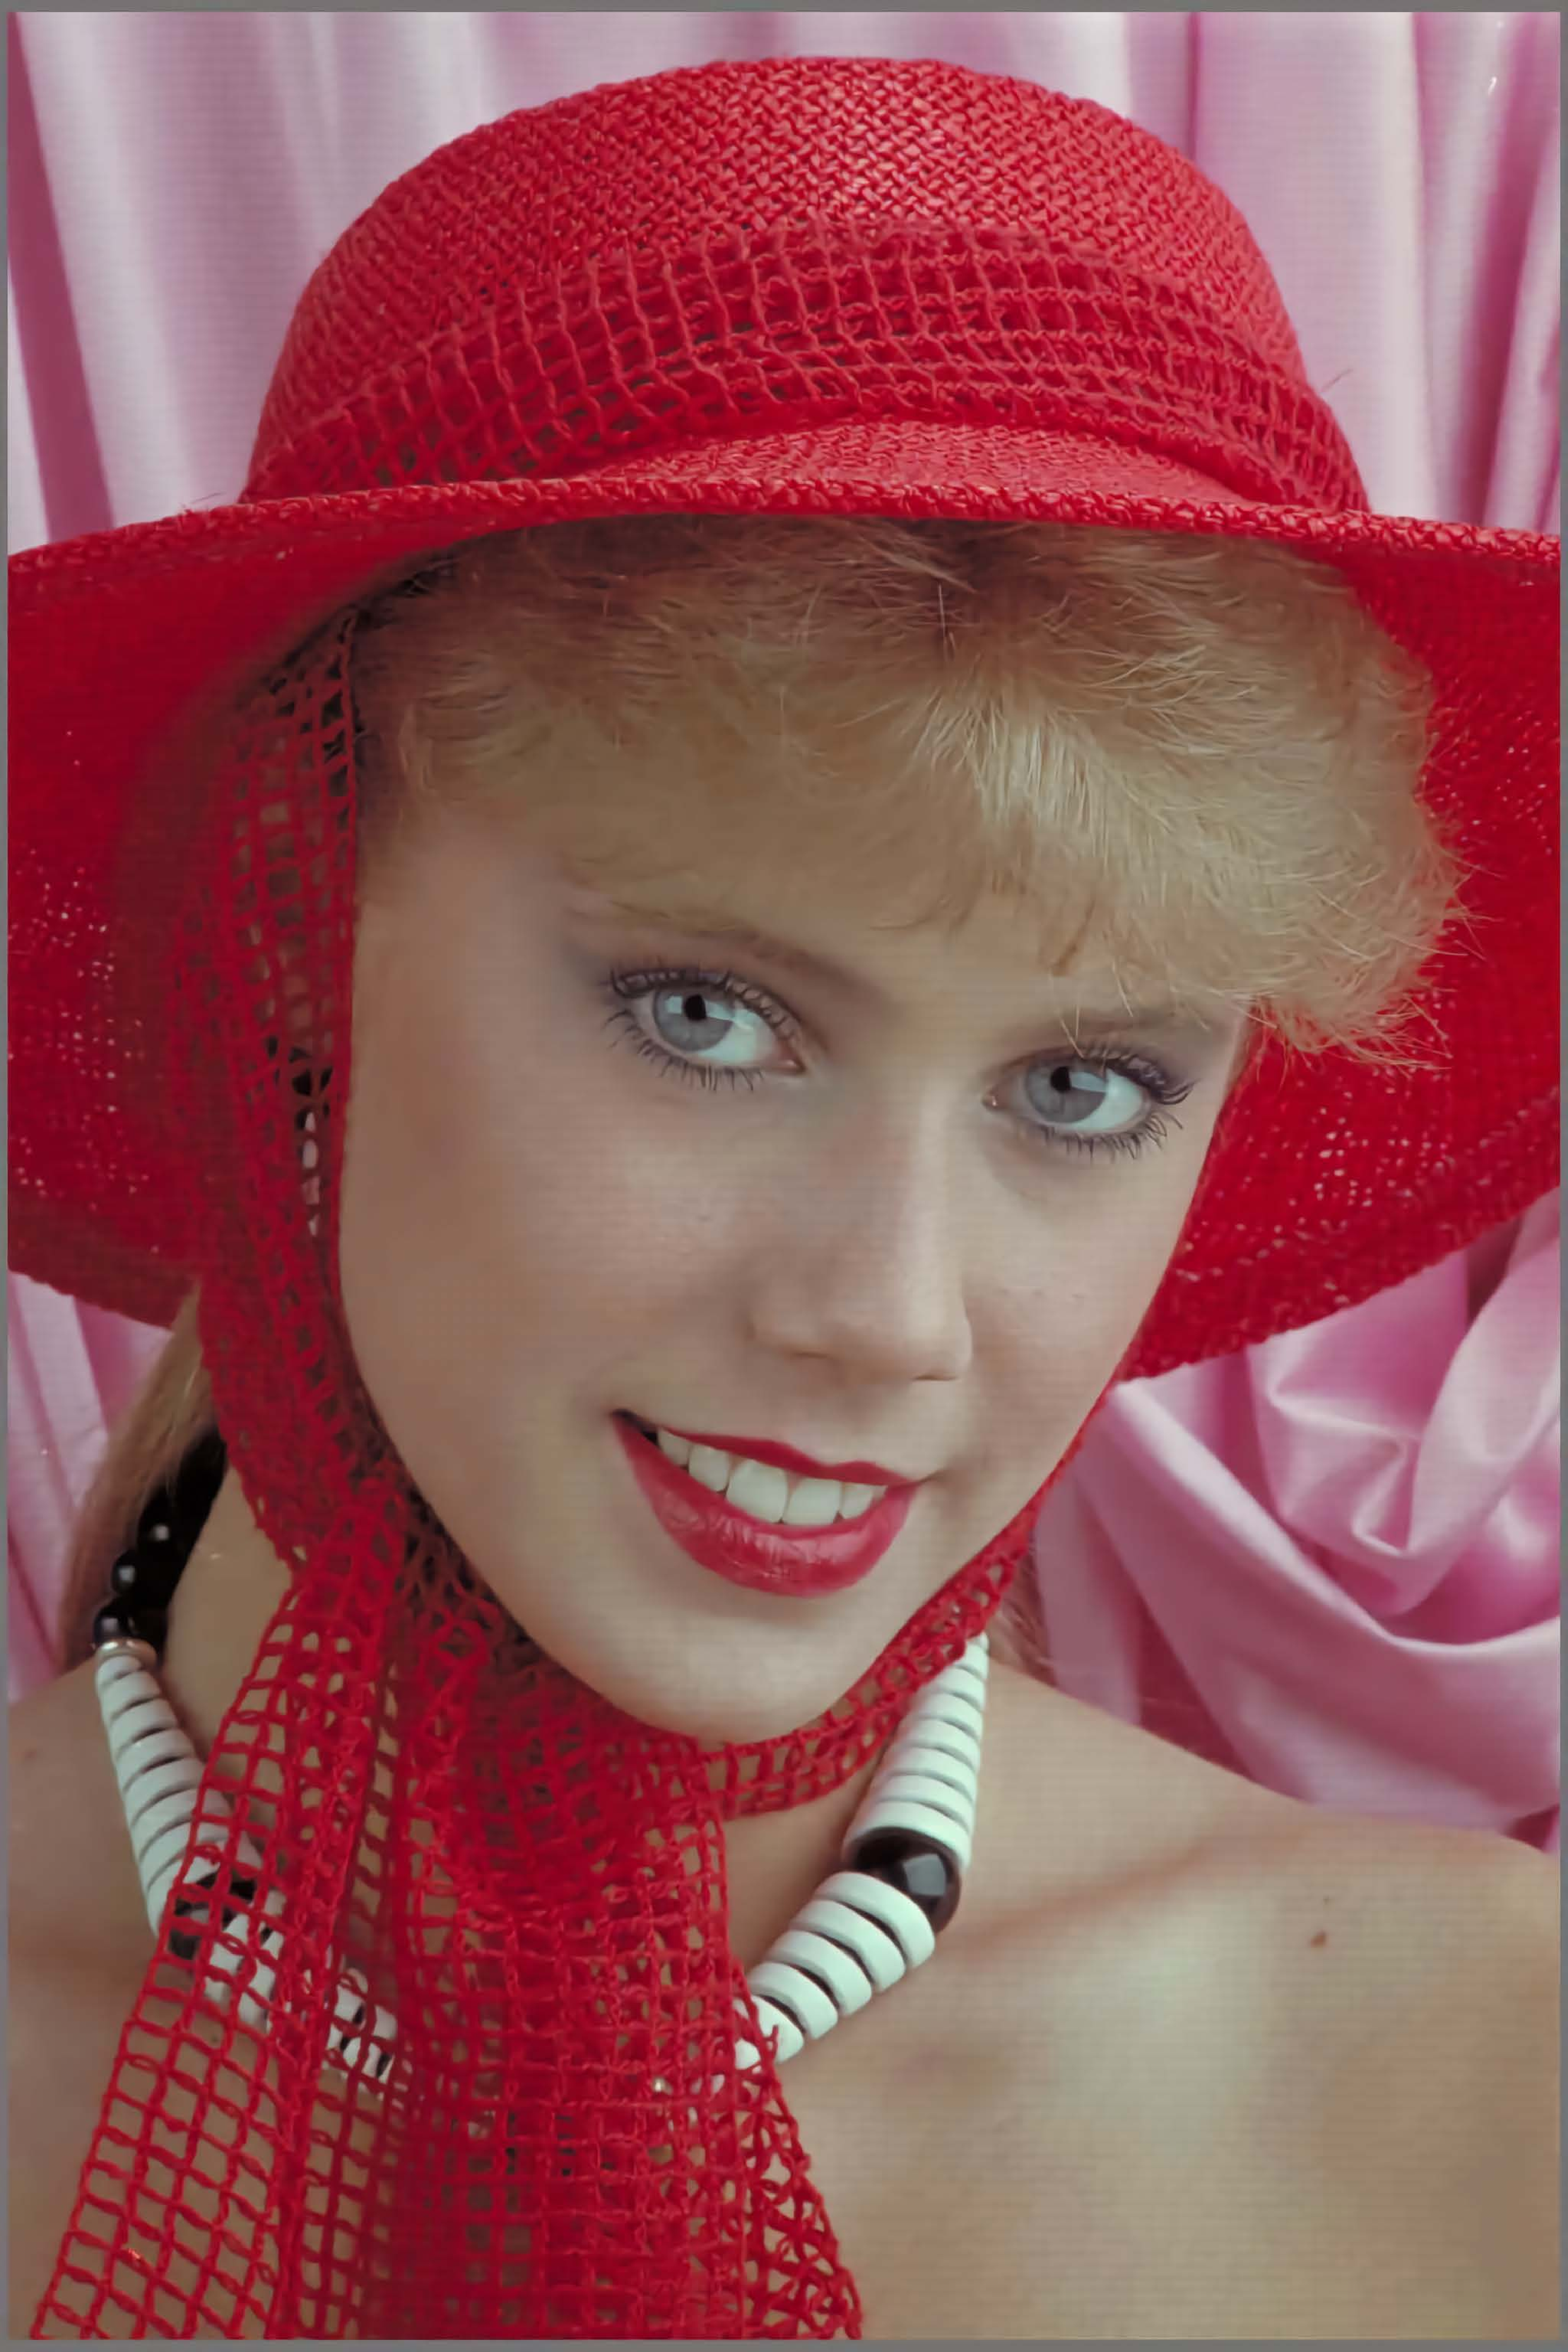
\includegraphics[width=\textwidth]{Immagini/IMAGES/mbt2018_2_IMG0004.pdf}
                \caption{Ballé 0.060bpp}
                \label{fig:ExampleBalle}
            \end{minipage}
            \begin{minipage}[]{0.13\linewidth}
                \centering
                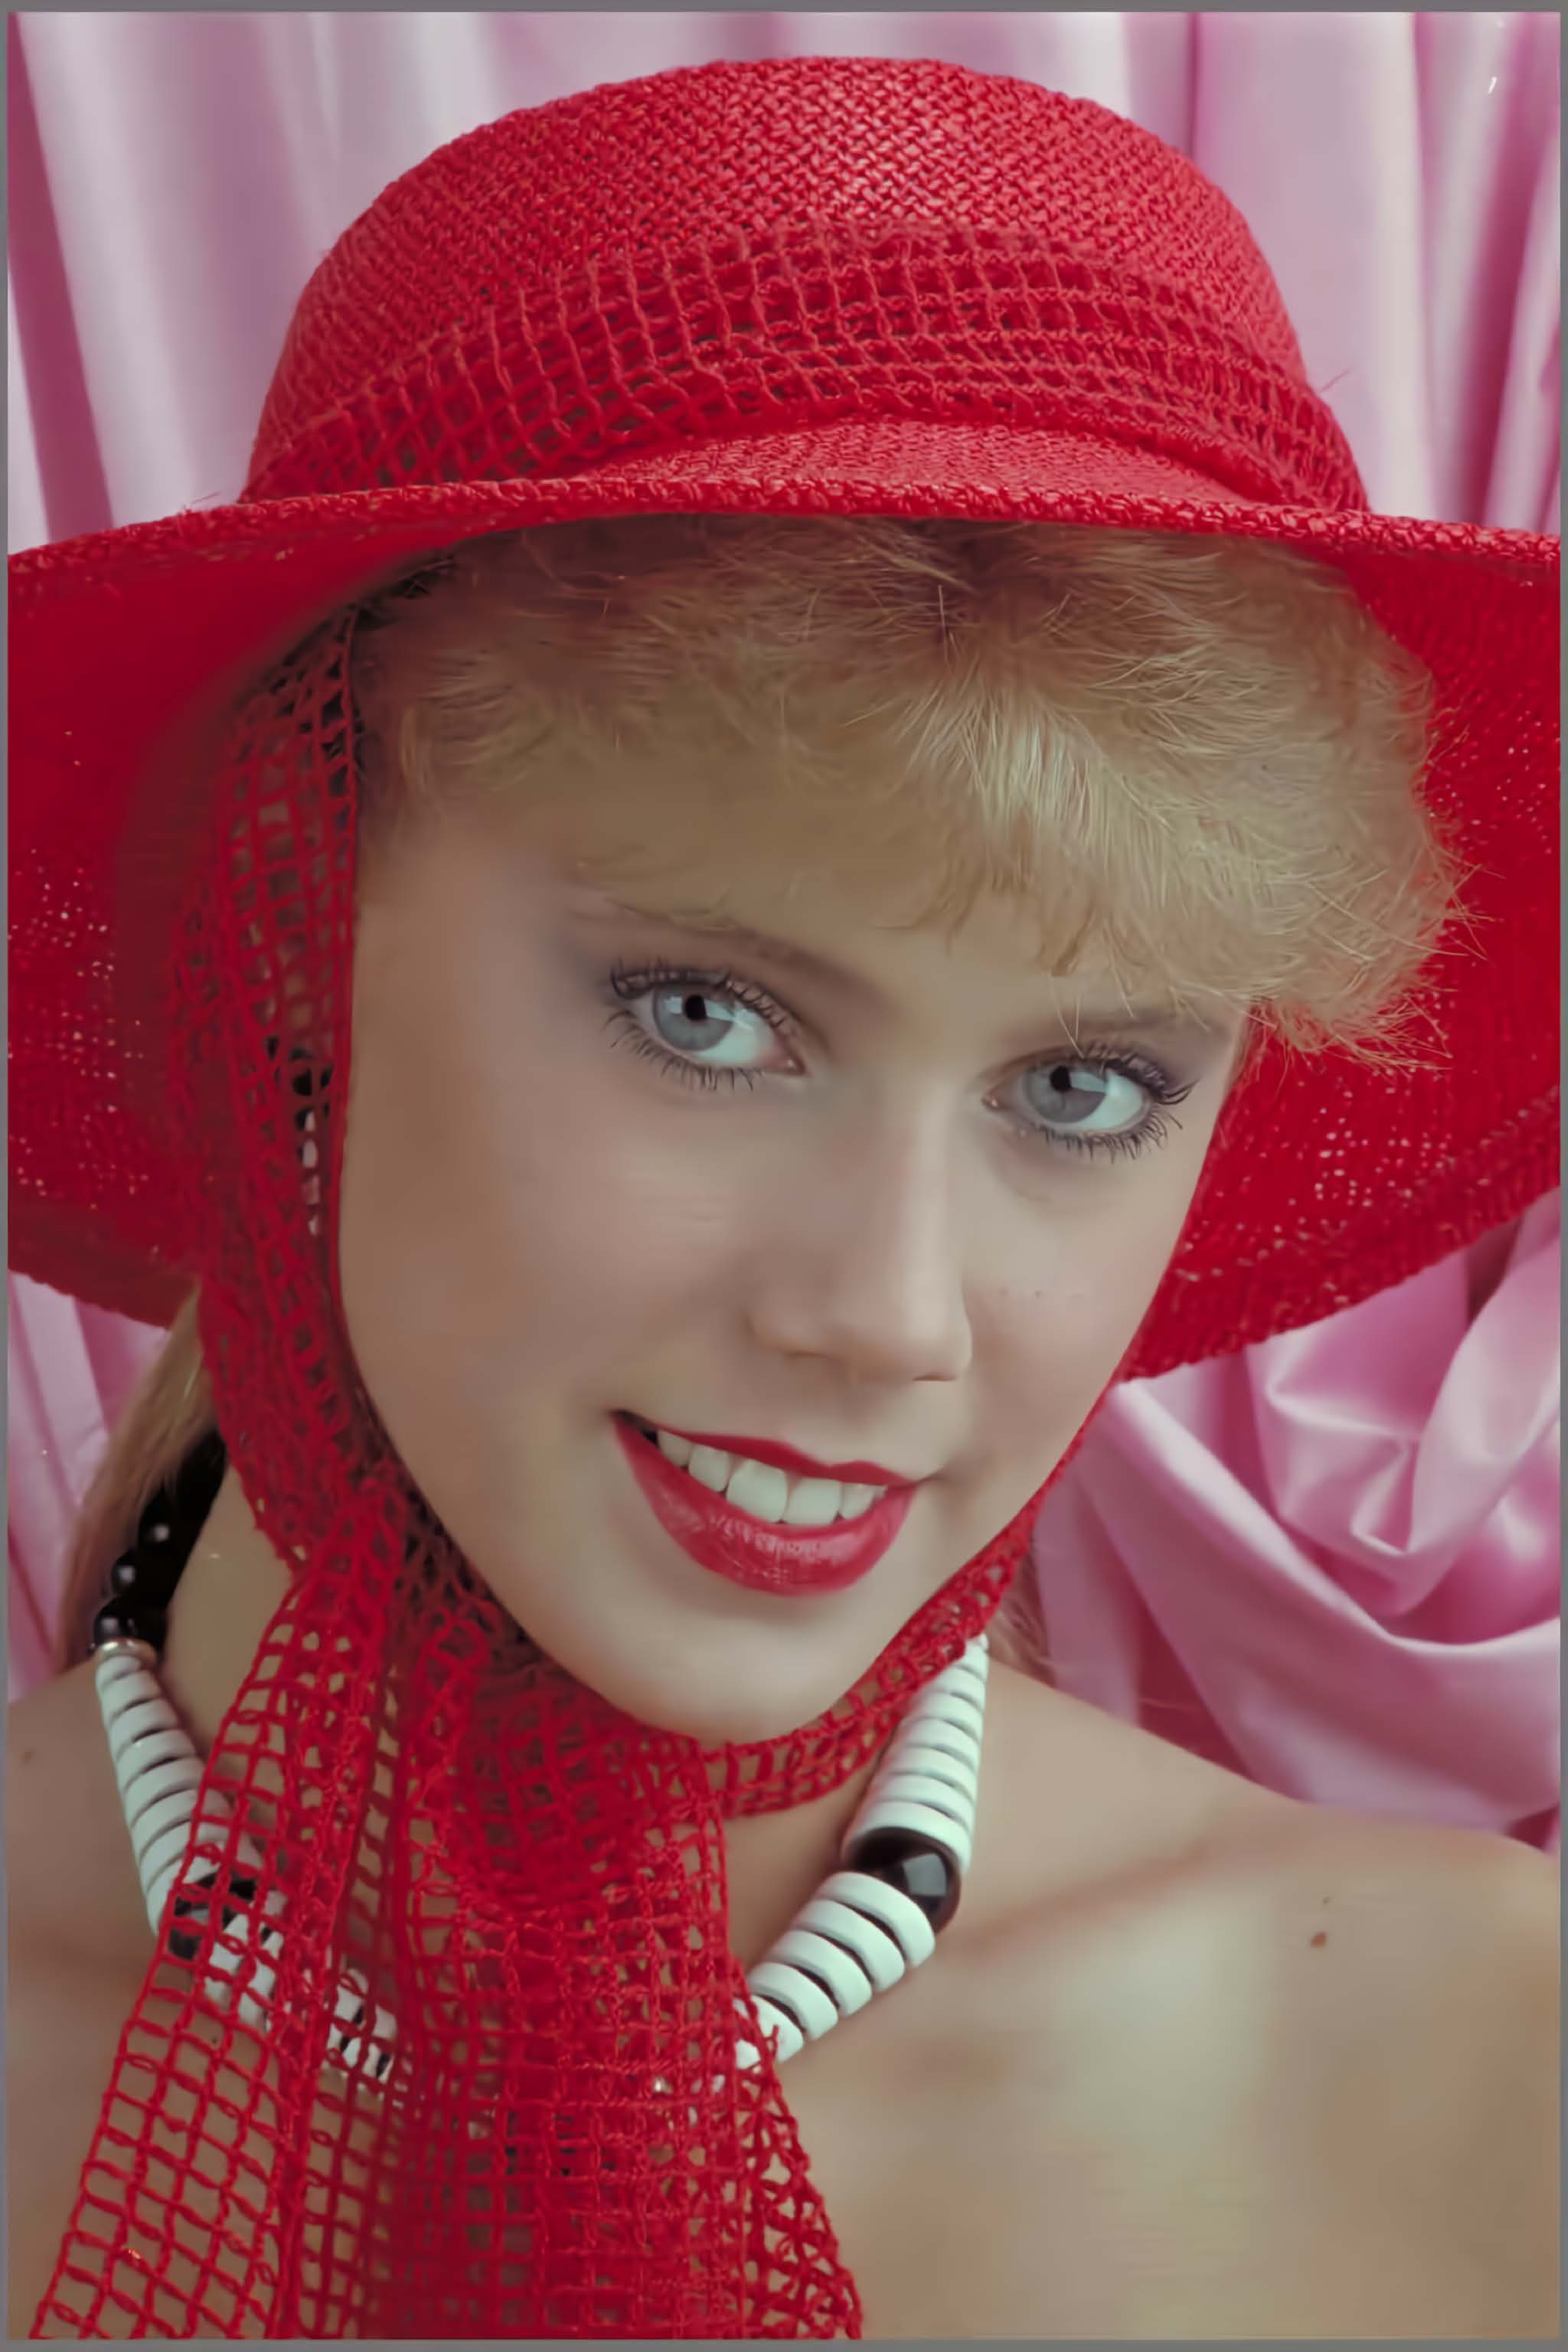
\includegraphics[width=\textwidth]{Immagini/IMAGES/cheng2020_attn_2_IMG0004.pdf}
                \caption{Cheng 0.056bpp}
                \label{fig:ExampleCheng}
            \end{minipage}
            \label{fig:ExamplesCompression}
        \end{figure}
        \footnotetext[1]{\fullcite{KodakDataset}}
    \end{frame}

    % \begin{frame}{Tempi di Compressione}
    %     \begin{figure}[t!]
    %         \centering
    %         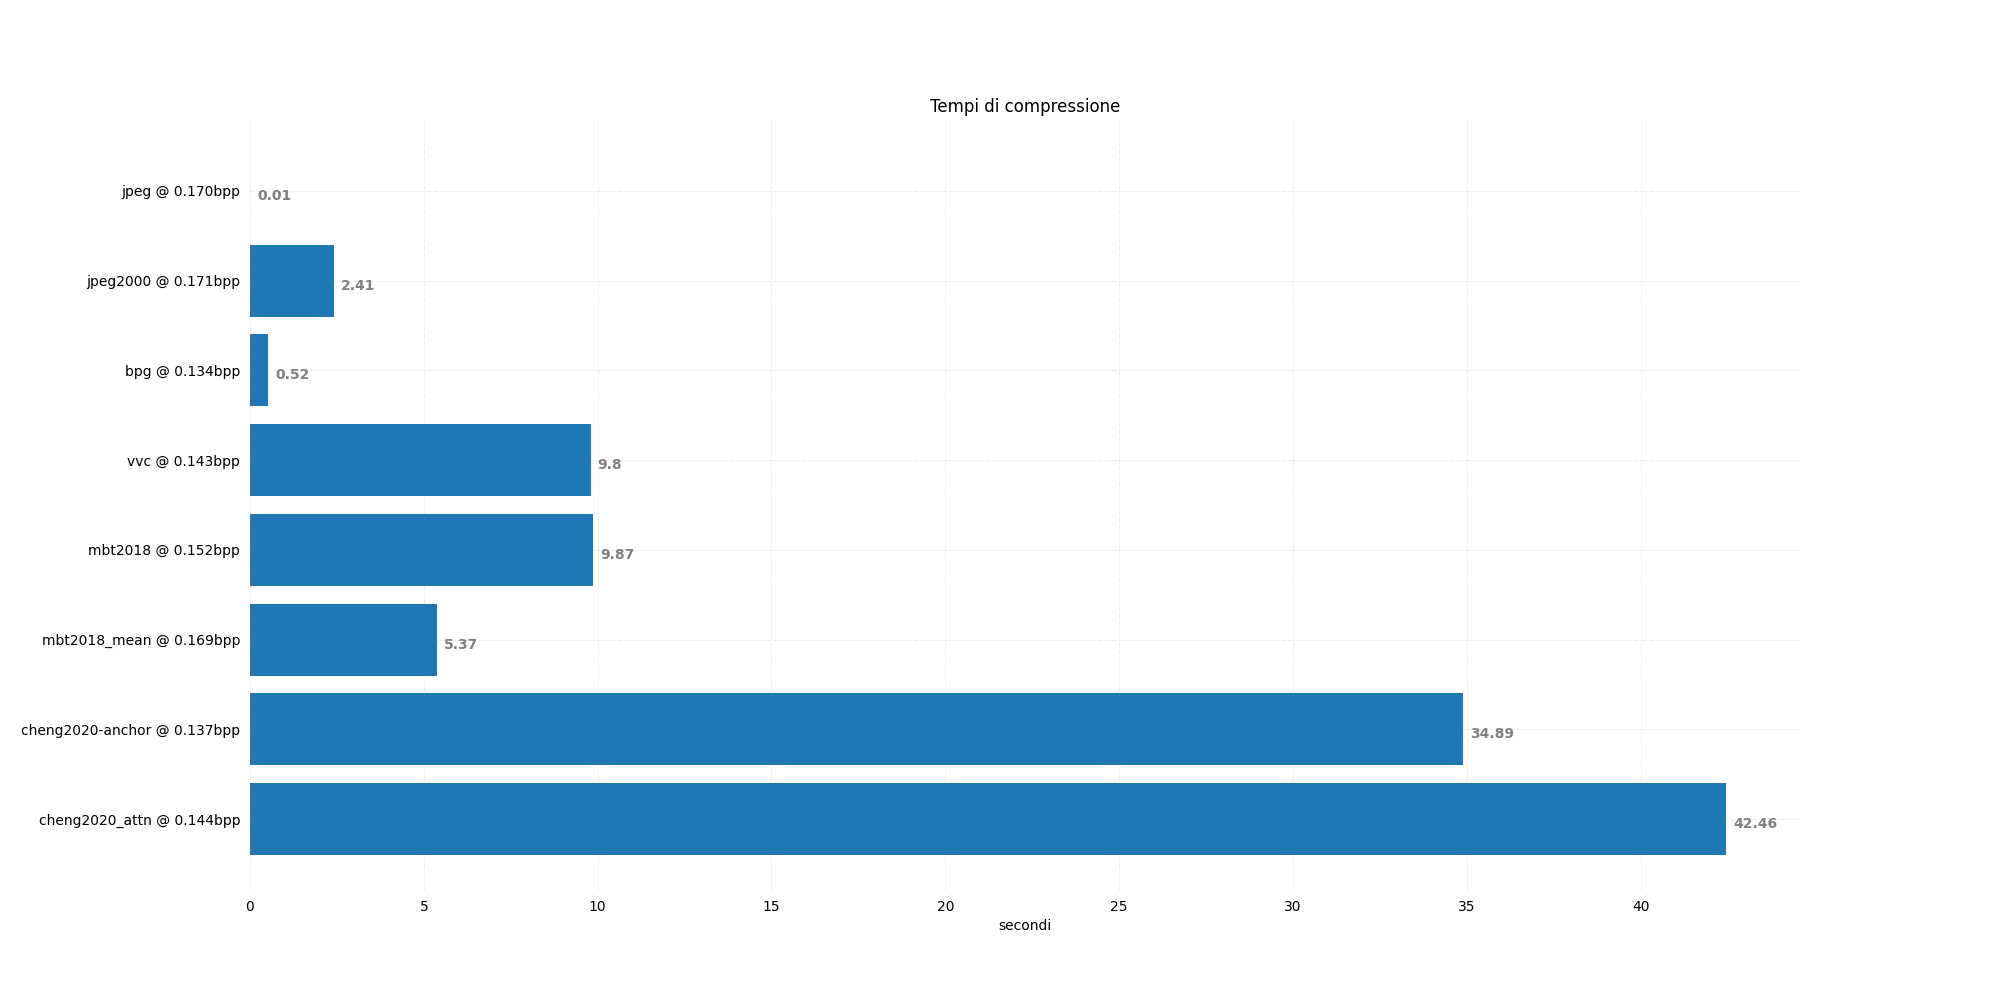
\includegraphics[width=1\textwidth]{Immagini/METRICS/times@0.16bpp.png}
    %         \caption{Tempi di compressione a 0.16 bpp}
    %         \label{fig:times16}
    %     \end{figure}
    % \end{frame}
    \begin{frame}{Tempi di Compressione}
        \begin{figure}[t!]
            \centering
            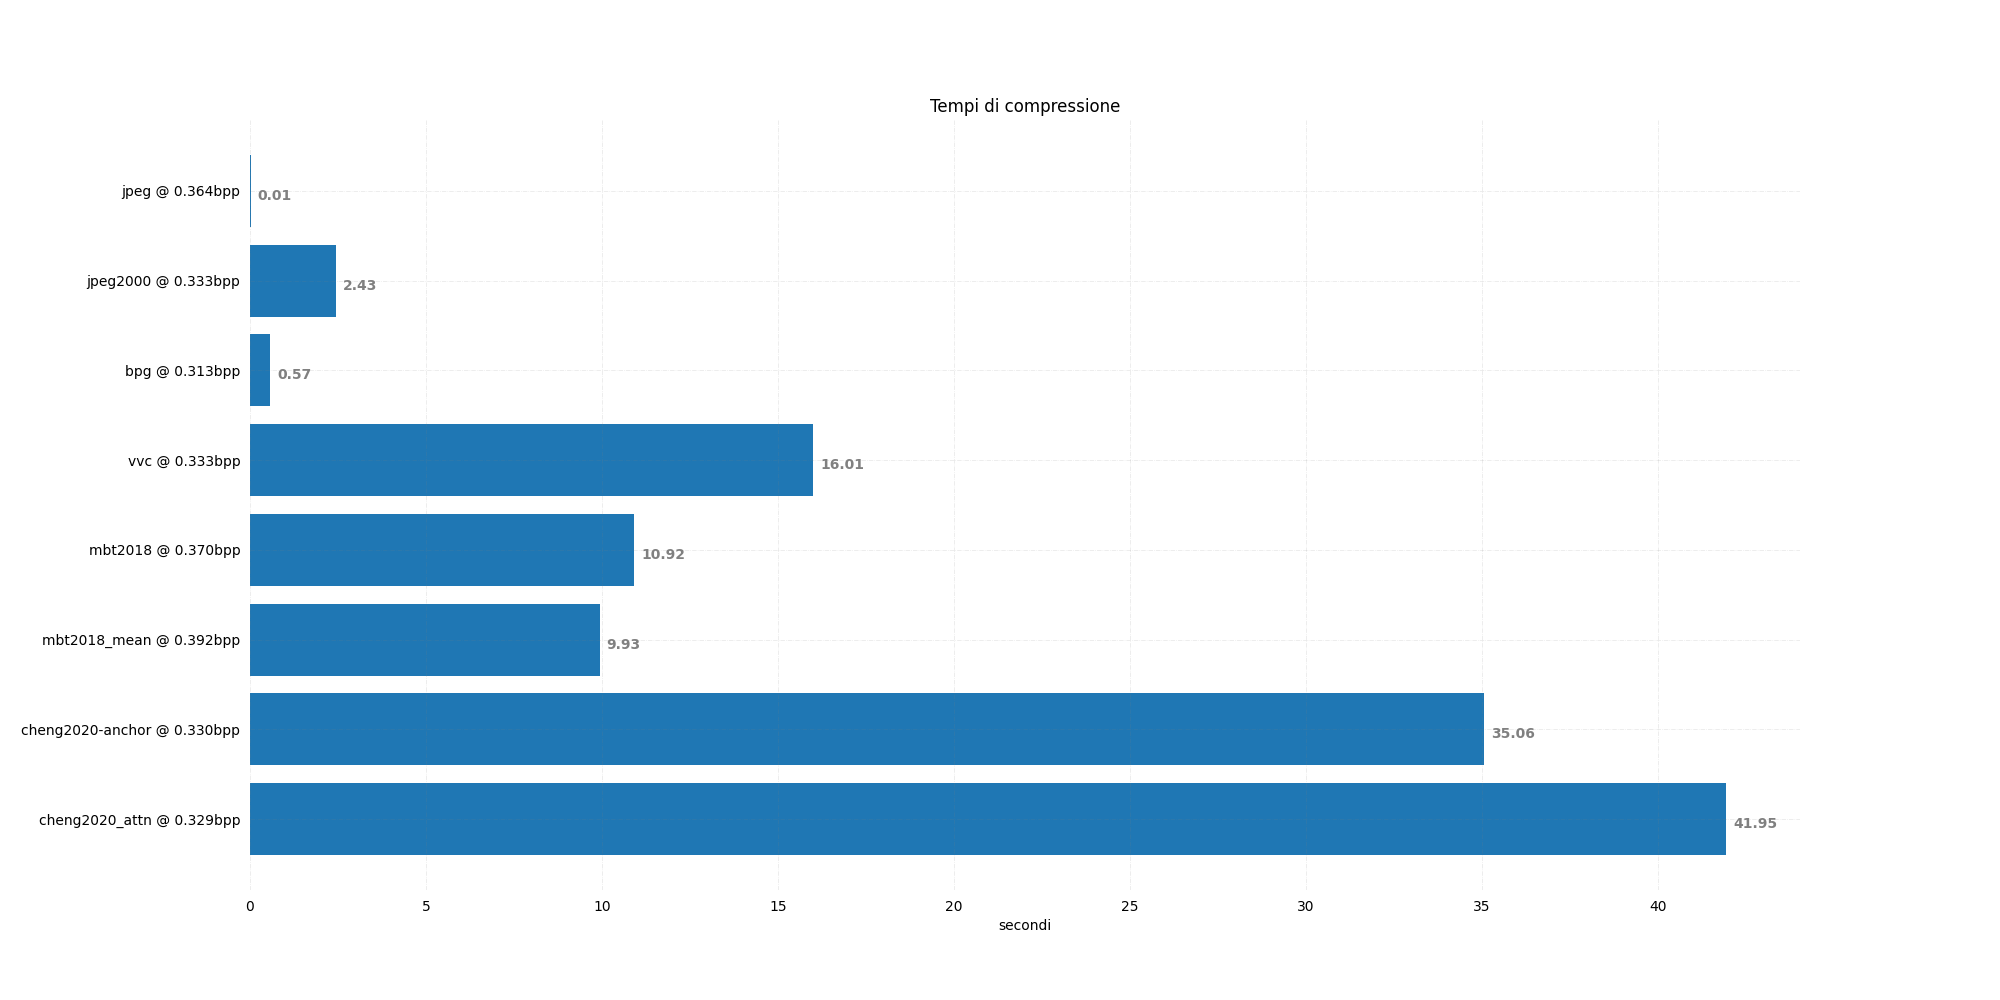
\includegraphics[width=1\textwidth]{Immagini/METRICS/times@0.34bpp.png}
            \caption{Tempi di compressione a 0.34 bpp}
            \label{fig:times34}
        \end{figure}
    \end{frame}

    \begin{frame}{PSNR}
        \begin{figure}[t!]
            \centering
            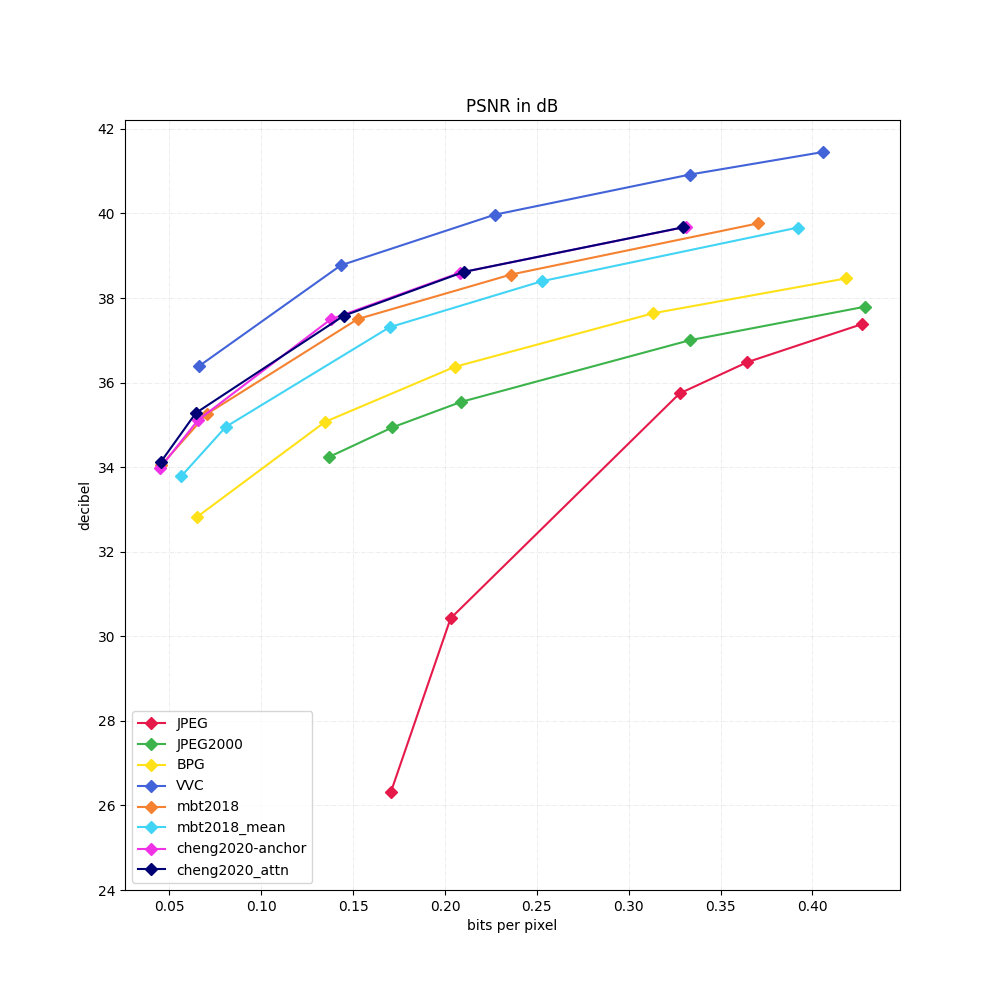
\includegraphics[width=0.57\textheight]{Immagini/METRICS/PSNR.png}
            \caption{Grafico del PSNR, punti corrispondenti alla media delle metriche sulle 24 immagini del dataset}
            \label{fig:GraphPSNR}
        \end{figure}
    \end{frame}

    \begin{frame}{MS-SSIM}
        \begin{figure}[t!]
            \centering
            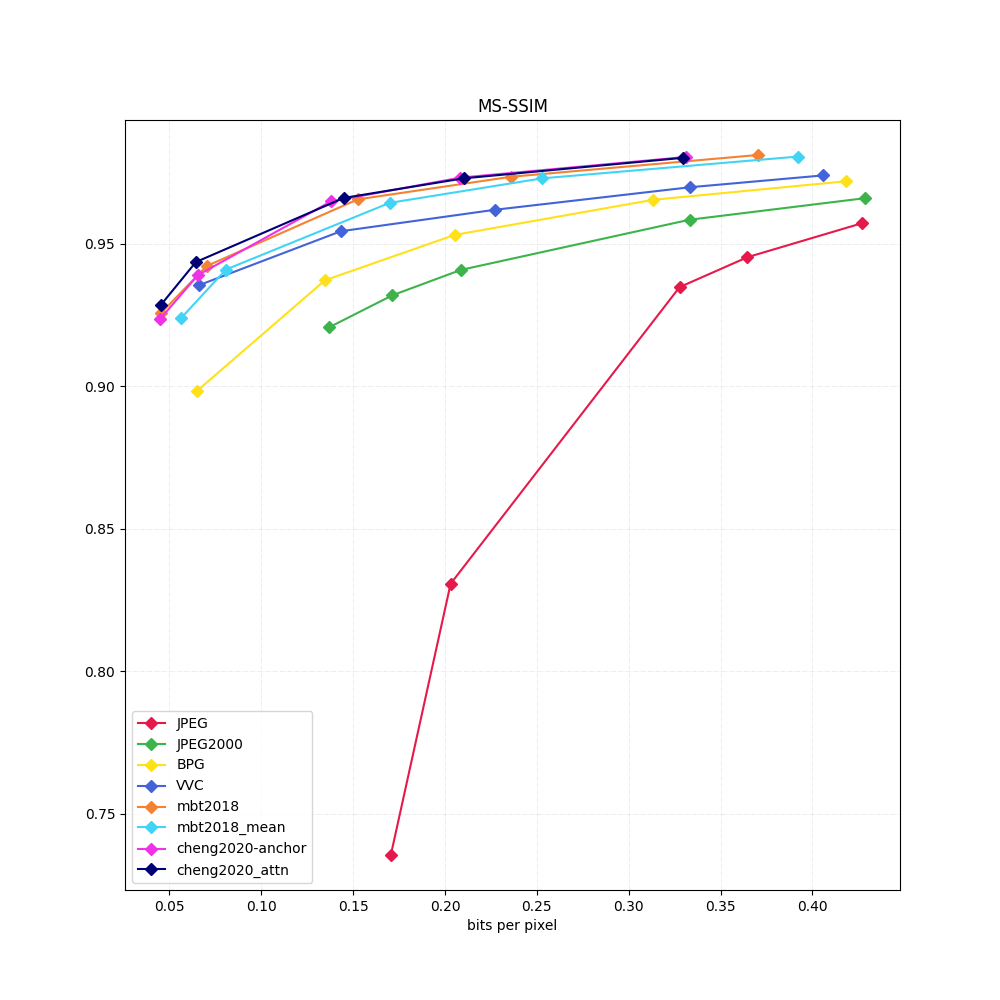
\includegraphics[width=0.57\textheight]{Immagini/METRICS/MS-SSIM.png}
            \caption{Grafico dell'MS-SSIM\footnotemark[1], punti corrispondenti alla media delle metriche sulle 24 immagini del dataset}
            \label{fig:GraphMS-SSIM}
        \end{figure}
        \footnotetext[1]{\fullcite{wang2003multiscale}}
    \end{frame}

    \begin{frame}{LPIPS}
        \begin{figure}[t!]
            \centering
            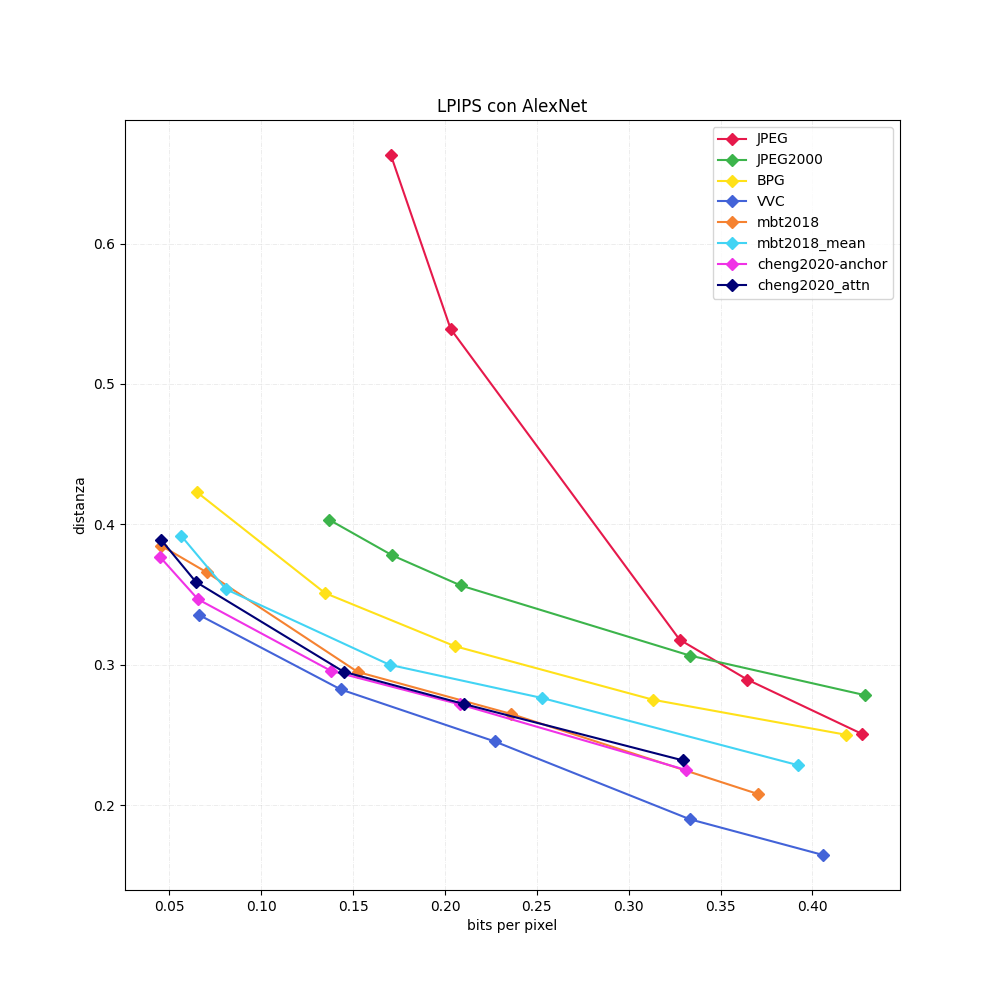
\includegraphics[width=0.57\textheight]{Immagini/METRICS/LPIPS.png}
            \caption{Grafico LPIPS\footnotemark[1] con AlexNet, punti corrispondenti alla media delle metriche sulle 24 immagini del dataset}
            \label{fig:GraphLPIPS}
        \end{figure}
        \footnotetext[1]{\fullcite{zhang2018unreasonable}}
    \end{frame}
    
    